\documentclass[12pt, a4paper]{article}

\usepackage[utf8]{inputenc}
\usepackage[english]{babel}
\usepackage{geometry}
\usepackage{csquotes}
\usepackage{graphicx}
\usepackage{blindtext}
\usepackage{amsthm}
\usepackage{amsmath}
\usepackage{amssymb}
\usepackage{amsfonts}
\usepackage{amsopn}
\usepackage{mathtools}
\usepackage{tikz}
\usepackage{authblk}
\usepackage{hyperref}
\usepackage{lipsum}
\usepackage{epstopdf}
\usepackage{algorithmic}
\usepackage{booktabs}
\usepackage[
    backend = biber,
    style   = alphabetic,
    sorting = anyvt,
]{biblatex}
\usepackage{enumitem}
\usepackage{pifont}
\usepackage{lineno}
\usepackage{arydshln}

\def\even{\mathrm{even}}
\def\odd{\mathrm{odd}}
\def\sym{\mathbf{sym}}
\def\tr{\mathrm{tr}}
\def\diag{\mathrm{diag}}
\def\sgn{\mathrm{sgn}}
\def\const{\mathrm{const.}}
\def\Var{\mathbb{V}\mathrm{ar}}
\def\Cov{\mathbb{C}\mathrm{ov}}
\def\mod_{\,\mathrm{mod}}
\def\id{\mathrm{id}}
\def\rank{\mathrm{rank}}
\def\argmin{\mathrm{argmin}}
\def\argmax{\mathrm{argmax}}
\def\fp{\,{:}\,} %Frobenius product


\renewcommand{\arraystretch}{1.5}
\addbibresource{references.bib}
\def\contra{
    \tikz[baseline, x=0.22em, y=0.22em, line width=0.032em]
    \draw (0,2.83)--(2.83,0) (0.71,3.54)--(3.54,0.71) (0,0.71)--(2.83,3.54) (0.71,0)--(3.54,2.83);
}

\renewcommand{\arraystretch}{1.5}
\addbibresource{references.bib}
\def\contra{
    \tikz[baseline, x=0.22em, y=0.22em, line width=0.032em]
    \draw (0,2.83)--(2.83,0) (0.71,3.54)--(3.54,0.71) (0,0.71)--(2.83,3.54) (0.71,0)--(3.54,2.83);
}

\renewcommand{\arraystretch}{1.5}
\addbibresource{references.bib}
\def\contra{
    \tikz[baseline, x=0.22em, y=0.22em, line width=0.032em]
    \draw (0,2.83)--(2.83,0) (0.71,3.54)--(3.54,0.71) (0,0.71)--(2.83,3.54) (0.71,0)--(3.54,2.83);
}

\renewcommand{\arraystretch}{1.5}
\addbibresource{references.bib}
\def\contra{
    \tikz[baseline, x=0.22em, y=0.22em, line width=0.032em]
    \draw (0,2.83)--(2.83,0) (0.71,3.54)--(3.54,0.71) (0,0.71)--(2.83,3.54) (0.71,0)--(3.54,2.83);
}

\renewcommand{\arraystretch}{1.5}
\addbibresource{references.bib}
\def\contra{
    \tikz[baseline, x=0.22em, y=0.22em, line width=0.032em]
    \draw (0,2.83)--(2.83,0) (0.71,3.54)--(3.54,0.71) (0,0.71)--(2.83,3.54) (0.71,0)--(3.54,2.83);
}

\renewcommand{\arraystretch}{1.5}
\addbibresource{references.bib}
\def\contra{
    \tikz[baseline, x=0.22em, y=0.22em, line width=0.032em]
    \draw (0,2.83)--(2.83,0) (0.71,3.54)--(3.54,0.71) (0,0.71)--(2.83,3.54) (0.71,0)--(3.54,2.83);
}

\renewcommand{\arraystretch}{1.5}
\addbibresource{references.bib}
\def\contra{
    \tikz[baseline, x=0.22em, y=0.22em, line width=0.032em]
    \draw (0,2.83)--(2.83,0) (0.71,3.54)--(3.54,0.71) (0,0.71)--(2.83,3.54) (0.71,0)--(3.54,2.83);
}


\renewcommand{\arraystretch}{1.5}
\addbibresource{references.bib}
\def\contra{
    \tikz[baseline, x=0.22em, y=0.22em, line width=0.032em]
    \draw (0,2.83)--(2.83,0) (0.71,3.54)--(3.54,0.71) (0,0.71)--(2.83,3.54) (0.71,0)--(3.54,2.83);
}

\newtheorem{theorem}{Theorem}[section]
\newtheorem{definition}[theorem]{Definition}
\newtheorem{lemma}[theorem]{Lemma}
\newtheorem{assumption}[theorem]{Assumption}
\newtheorem{proposition}[theorem]{Proposition}
\newtheorem{result}[theorem]{Result}
\newtheorem{corollary}[theorem]{Corollary}
\newtheorem{conjecture}[theorem]{Conjecture}
\newtheorem*{theorem*}{Theorem}
\newtheorem*{remark}{Remark}
\newtheorem*{example}{Example}

% Width
\addtolength{\oddsidemargin}{-0.375in}
\addtolength{\evensidemargin}{-0.375in}
\addtolength{\textwidth}{0.75in}

% Height
\addtolength{\topmargin}{-0.375in}
\addtolength{\textheight}{0.75in}
% Boris
\definecolor{teal}{rgb}{0.14, 0.78, 0.65}
\def\BA#1{\textcolor{teal}{BA: #1}}

% Patrick
\definecolor{gold}{rgb}{0.78, 0.65, 0.14}
\def\PF#1{\textcolor{gold}{PF: #1}}

\usetikzlibrary{shapes, arrows}

\tikzstyle{0} = [rectangle, draw = blue!00, fill = blue!20, very thick, text width = 2cm, text centered, rounded corners]
\tikzstyle{1} = [rectangle, draw = green!00, fill = green!20, very thick, text width = 4.5cm, text centered, rounded corners]
\tikzstyle{2} = [rectangle, draw = yellow!00, fill = yellow!20, very thick, text width = 4.5cm, text centered, rounded corners]
\tikzstyle{3} = [rectangle, draw = orange!00, fill = orange!20, very thick, text width = 4.5cm, text centered, rounded corners]
\tikzstyle{4} = [rectangle, draw = red!00, fill = red!20, very thick, text width = 4.5cm, text centered, rounded corners]

\tikzstyle{arrow} = [draw, ->, thick]

\def\contra{
    \tikz[baseline, x = 0.22em, y=0.22em, line width = 0.032em]
    \draw (0,2.83)--(2.83,0) (0.71,3.54)--(3.54,0.71) (0,0.71)--(2.83,3.54) (0.71,0)--(3.54,2.83);
}


\title{Numerical Bifurcation Analysis for Heat Transfer by the Edge Plasma of a Tokamak}
\author{Boris Andrews}
\affil{Mathematical Institute, University of Oxford}
\date{March 2022}



\begin{document}
    \pagenumbering{gobble}
    \maketitle
    
    
    
    \begin{abstract}
        \BA{Abstract.}
    \end{abstract}
    
    
    
    \newpage
    \tableofcontents
    \BA{I'm aware having a contents page is ridiculous, it's just nice to have for now for navigation purposes.}
    
    
    
    \newpage
    \pagenumbering{arabic}
        \chapter{Introduction}
    \BA{Introduction.}
    
    \BA{Motivation.}
    
    \BA{Previous work and literature review.}
    
    \BA{Results we might expect to find.}
    
    \BA{Relevance and impact.}
    
    \BA{Other topics to note mentioned on the transfer thesis requirements.}

    \BA{One thing I need to generally do is scan through to find any times I've used ``-ise'' and change them to ``-ize''- a good habit! :( Also should do the same for ``modelling'' to ``modeling'', as well as ``behaviour'' to ``behavior'' (or pretty much anything as suggested by Grammarly).}

    \BA{Remove all "we"s and "us"s- passive voice!}


    \renewcommand{\arraystretch}{1.5}
\addbibresource{references.bib}
\def\contra{
    \tikz[baseline, x=0.22em, y=0.22em, line width=0.032em]
    \draw (0,2.83)--(2.83,0) (0.71,3.54)--(3.54,0.71) (0,0.71)--(2.83,3.54) (0.71,0)--(3.54,2.83);
}

    \renewcommand{\arraystretch}{1.5}
\addbibresource{references.bib}
\def\contra{
    \tikz[baseline, x=0.22em, y=0.22em, line width=0.032em]
    \draw (0,2.83)--(2.83,0) (0.71,3.54)--(3.54,0.71) (0,0.71)--(2.83,3.54) (0.71,0)--(3.54,2.83);
}


    
    \section*{Summary}
        \BA{Summary.}

        \chapter{Physical Model and System of Equations}
    \BA{Introduction.}
    
    \BA{Room for lots of pictures here.}
    
    \BA{What physics characterise a (magnetised) neutral plasma? Quasi-neutral mix of \emph{separated} electrically-charged phases. (Check out the \href{https://en.wikipedia.org/wiki/Plasma_(physics)}{plasma Wikipedia page}.)}
    
    \BA{Creates a coupled system with the EM field.}
    
    \BA{What causes a fluid to turn into a plasma? Ionisation. (High heat/strong EM field.)}
    
    \BA{What makes a tozmahok plasma special (give stats):
    \begin{itemize}
        \item  \emph{Massive} heat.
        \item  \emph{Massive} magnetic field- highly magnetised. (Talk about particle gyro-orbits and drifts.)
        \item  \emph{Minimal} density. (Why?)
    \end{itemize}.}
    
    \BA{Will make the assumptions:
    \begin{itemize}
        \item  Only 2 phases (positive and negative) i.e.:
        \begin{itemize}
            \item  The plasma is fully ionised, i.e. neutrals (or at least the effects thereof) are negligible. I've been led to believe this is generally the case in edge plasmas (i.e. outside the divertor). (A bold assumption?)
            \item  Dust and impurities (or at least the effects thereof) are negligible. (A bold assumption?)
        \end{itemize}
        \item  Only (thermalising) Coulomb collisions are considered- these are generally dominant over the others in a tozmahok. (N.B. No fusion.)
        \item  Relativistic effects are negligible. (Is observing that the velocity scale is much smaller than $c$ sufficient justification? Imperial guy at the NEPTUNE workshop appeared to think not.)
    \end{itemize}}
    
    \BA{Complicated BCs in a tozmahok.}
    
    \begin{figure}[!h]
        \centering
        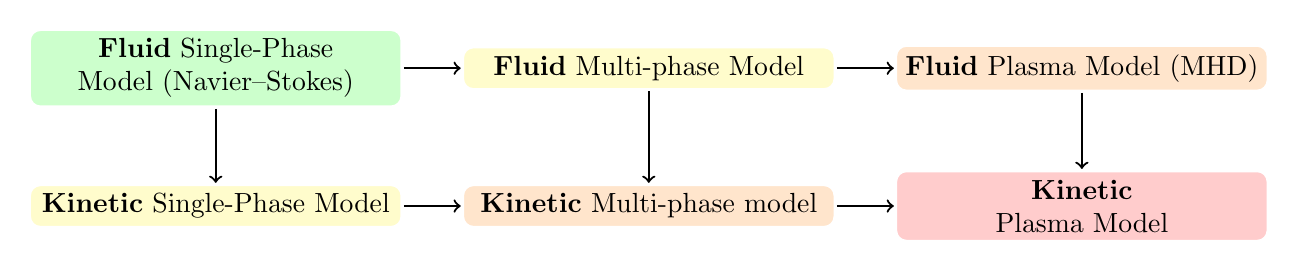
\begin{tikzpicture}[align = center, node distance = 4cm, auto]
            \node[1] (11) at (0, 0) {{\bf Fluid} Single-Phase Model (Navier–Stokes)};
            \node[2] (12) at (0, -1.75) {{\bf Kinetic} Single-Phase Model};
            \node[2] (21) at (5.5, 0) {{\bf Fluid} Multi-phase Model};
            \node[3] (22) at (5.5, -1.75) {{\bf Kinetic} Multi-phase model};
            \node[3] (31) at (11, 0) {{\bf Fluid} Plasma Model (MHD)};
            \node[4] (32) at (11, -1.75) {{\bf Kinetic} \\ Plasma Model};
    
            \path[arrow] (11) -- (12);
            \path[arrow] (11) -- (21);
            \path[arrow] (12) -- (22);
            \path[arrow] (21) -- (22);
            \path[arrow] (21) -- (31);
            \path[arrow] (22) -- (32);
            \path[arrow] (31) -- (32);
        \end{tikzpicture}
        \caption{\BA{Diagram of workflow for creating a kinetic plasma model to account for pressure anisotropy.}}
    \end{figure}
    
    
    \section{Kinetic Models}
        \BA{What is a ``kinetic'' model.}
        
        \subsection{Single-Phase Fluids}
            \BA{The resultant kinetic PDE. (Boltzmann equation.)}
                        
            \BA{How we traditionally convert that to a ``fluid'' model.}
            
            \BA{Will use this simpler case as a reference study to develop the ideas for the more complicated tozmahok plasma case.}

        \subsection{Multiphase Fluids}
            \BA{Similar analysis for a multiphase fluid, in preparation for handling the tozmahok plasmas.}
        
        \subsection{Tozmahok Plasmas}
            \BA{Why the fluid/MHD model reductions aren't necessarily valid in tozmahok plasmas. (Incorrectly assumed dominant collisional term- get some estimates on the scale of these terms in the edge plasma. Good content under ``Mathematical Descriptions'' \href{https://en.wikipedia.org/wiki/Plasma_(physics)}{here}.)}
            
            \BA{Many effects not captured my MHD/2 fluid models (check out \href{https://upload.wikimedia.org/wikipedia/commons/a/a9/A_Comparison_Chart_For_Modeling_Plasma2.png}{this} diagram off Wikipedia, or again the content under ``Mathematical Descriptions'' \href{https://en.wikipedia.org/wiki/Plasma_(physics)}{here}.):
            \begin{itemize}
                \item  Most plasma waves
                \item  Most plasma/kinetic instabilities
                \item  Landau damping/bump-on-tail instability
                \item  Leakage
                \item  Structures (Beams/Double layers)
                \item  Anisotropic pressure
            \end{itemize}}
            
            \BA{The resultant kinetic PDE. (Boltzmann/Vlasov equations.)}
            
            \BA{Talk about gyrokinetic model:
            \begin{itemize}
                \item  The model's physical basis/mathematics. (Equations provide good insight into the origin of some behavioural effects, e.g. gyro-orbits/drifts.)
                \item  Why we don't use it on the general kinetic equation:
                \begin{itemize}
                    \item  High mathematical (more terms in lower dimensions doesn't necessarily mean faster computation)/computational (really don't want to do a 5D simulation) complexity.
                    \item  Errors from neglection of terms. (Non-physical behaviour over long times/resonances and adiabatic invariants can be lost.)
                \end{itemize}
                \item  We \emph{will} however use it for the PIC correction.
            \end{itemize}}
    
    
    \section{Coupled Maxwellian/Correction Decomposition}
        \BA{How we can re-adapt the techniques that traditionally give a fluid model when the collision operator is non-dominant to get an accurate fluid model, to apply modern techniques in fluid simulation?}
        
        \BA{Expand as a sum of a Maxwellian and some correction!}
        
        \subsection{Maxwellian Background: A \emph{Fluid} Model}
            \BA{Ideas already well-developed!}
            
            \BA{Correction contribution not too problematic (hopefully).}
            
        \subsection{Anisotropic Correction: A \emph{Kinetic} Model}
            \BA{Not just kicking the problem down the road- plasma is thermalised/Maxwellian in ``most places'' for ``most physically relevant simulations'', so the correction is (compartively) small in ``most places''.}
            
            \BA{How do we model this:
            \begin{itemize}
                \item  Lattice Boltzmann?
                \item  Some series expansion?
                \item  Particle-in-cell (PIC)?
            \end{itemize}}
    
    
    \section{Edge Plasma Model}
        \BA{Little about the edge plasma model we're going to consider:
        \begin{itemize}
            \item  Looking for symmetric structures on a low aspect ratio?
            \item  Idk there's a lot of ways to consider this- I could very well end up doing different kinds of simulations with all different kinds of BCs in the final product, and seeing how my results match up.
        \end{itemize}}

    \section*{Summary}
        \BA{Summary.}
        \chapter{Numerical Simulation and Preconditioning}
    \BA{Introduction.}
    
    
    \renewcommand{\arraystretch}{1.5}
\addbibresource{references.bib}
\def\contra{
    \tikz[baseline, x=0.22em, y=0.22em, line width=0.032em]
    \draw (0,2.83)--(2.83,0) (0.71,3.54)--(3.54,0.71) (0,0.71)--(2.83,3.54) (0.71,0)--(3.54,2.83);
}

    \renewcommand{\arraystretch}{1.5}
\addbibresource{references.bib}
\def\contra{
    \tikz[baseline, x=0.22em, y=0.22em, line width=0.032em]
    \draw (0,2.83)--(2.83,0) (0.71,3.54)--(3.54,0.71) (0,0.71)--(2.83,3.54) (0.71,0)--(3.54,2.83);
}


    
    \section*{Summary}
        \BA{Summary.}
        \section{Bifurcation Analysis}
    \BA{Lots to be said about the search for symmetry and ill-posedness here.}

    \BA{Also worthy of note is the fact that the way I handle the PIC side could end up being non-deterministic, which would maybe mess up the deflation algorithm. (Maybe use some kind of deterministic seed- I could run the bifurcation analysis a few times with different seeds, and compare the results?)}
        \section{Summary and Further Work}
    
    
    
    %\section{}
    \newpage
    \pagenumbering{gobble}
        \printbibliography
\end{document}
